\newsection
\subsection{Interpretability}
\label{sec:interpretability}
\sectionauthors{John Hewitt*, Armin W. Thomas*, Pratyusha Kalluri, Rodrigo Castellon, Christopher D. Manning}

Compared to most other machine learning models, foundation models are characterized by a vast increase in training data and complexity and the emergence of unforeseen capabilities: foundation models are able to do unforeseen tasks and do these tasks in unforeseen ways.
The increasing adoption of foundation models thereby creates growing desires, demands, and unprecedented challenges for understanding their behavior.

In contrast to task-specific models, foundation models are trained across vast and highly disparate datasets, potentially spanning many domains and modalities (see \refsec{training}).
Through this training, foundation models learn an exceptionally wide range of behaviors, which can vary profoundly between tasks and domains, as demonstrated by their ability to be adapted to many different types of downstream tasks and to exhibit behaviors that are specific for each of these tasks (see \refsec{adaptation}).
Take GPT-3 as an example, which was trained as one huge model to simply predict the next word in a text.
While this is a very specific and simple-to-define learning task, it has enabled GPT-3 to gain capabilities that far exceed those that one would associate with next word prediction, by combining it with a vast training dataset that comprises all kinds of internet text.
As a result, GPT-3 can now adapt behaviors that are clearly outside of the scope of its original training task, such as simple arithmetic and computer programming, when provided with few training samples.
This demonstrates that it is challenging to answer even the seemingly simplest question about a foundation model: what capabilities does it have?

Moreover, it is an open question to what extent these diverse capabilities rely on distinct or shared \textit{model mechanisms}, akin to algorithmic building blocks within the model.
On the one hand, foundation models can be interpreted as single models, which utilize some set of generalizable model mechanisms to perform well across tasks and domains.
In this case, a full understanding of their behavior can be gained by identifying and characterising these mechanisms.
On the other hand, the ability of foundation models to adapt profoundly distinct behaviors for different tasks suggests that they can also be understood as a large collection of independent expert models, each tailored to a specific task.
For example, it seems unlikely that the model parameters that GPT-3 uses to do arithmetic could have much to do with the parameters used to translate from English to French. 
In this case, explanations of model behavior in one task are therefore not necessarily informative about behavior in other tasks.
We refer to this as the \emph{one model-many model} nature of foundation models (see \reffig{intrp}) and argue that understanding where foundation models are located on this spectrum between one and many models will be central to understanding their behavior.

Toward systematizing this area of study, we present and discuss three levels of understanding foundation models
~\citep[inspired by][]{marr1982vision}:
in simple terms, we first discuss the challenges and opportunities in understanding \textit{what} a model is capable of doing, then \textit{why} it outputs certain behaviors, and lastly \textit{how} it does it.
Specifically, questions of \emph{`what'} aim to characterize the kinds of behaviors that a model can perform without ``peeking inside" the model, while questions of \emph{`why'} aim to provide explanations of the model's behaviors in terms of potential causes in the data, and questions of \emph{`how'} aim to understand the internal model representations and mechanisms that produce these behaviors.
After presenting all three levels, we conclude by discussing potential consequences resulting from the non-interpretability and interpretability of foundation models.


% Chris suggested to move the figure to the second page
\begin{figure}[!ht]
    \centering
    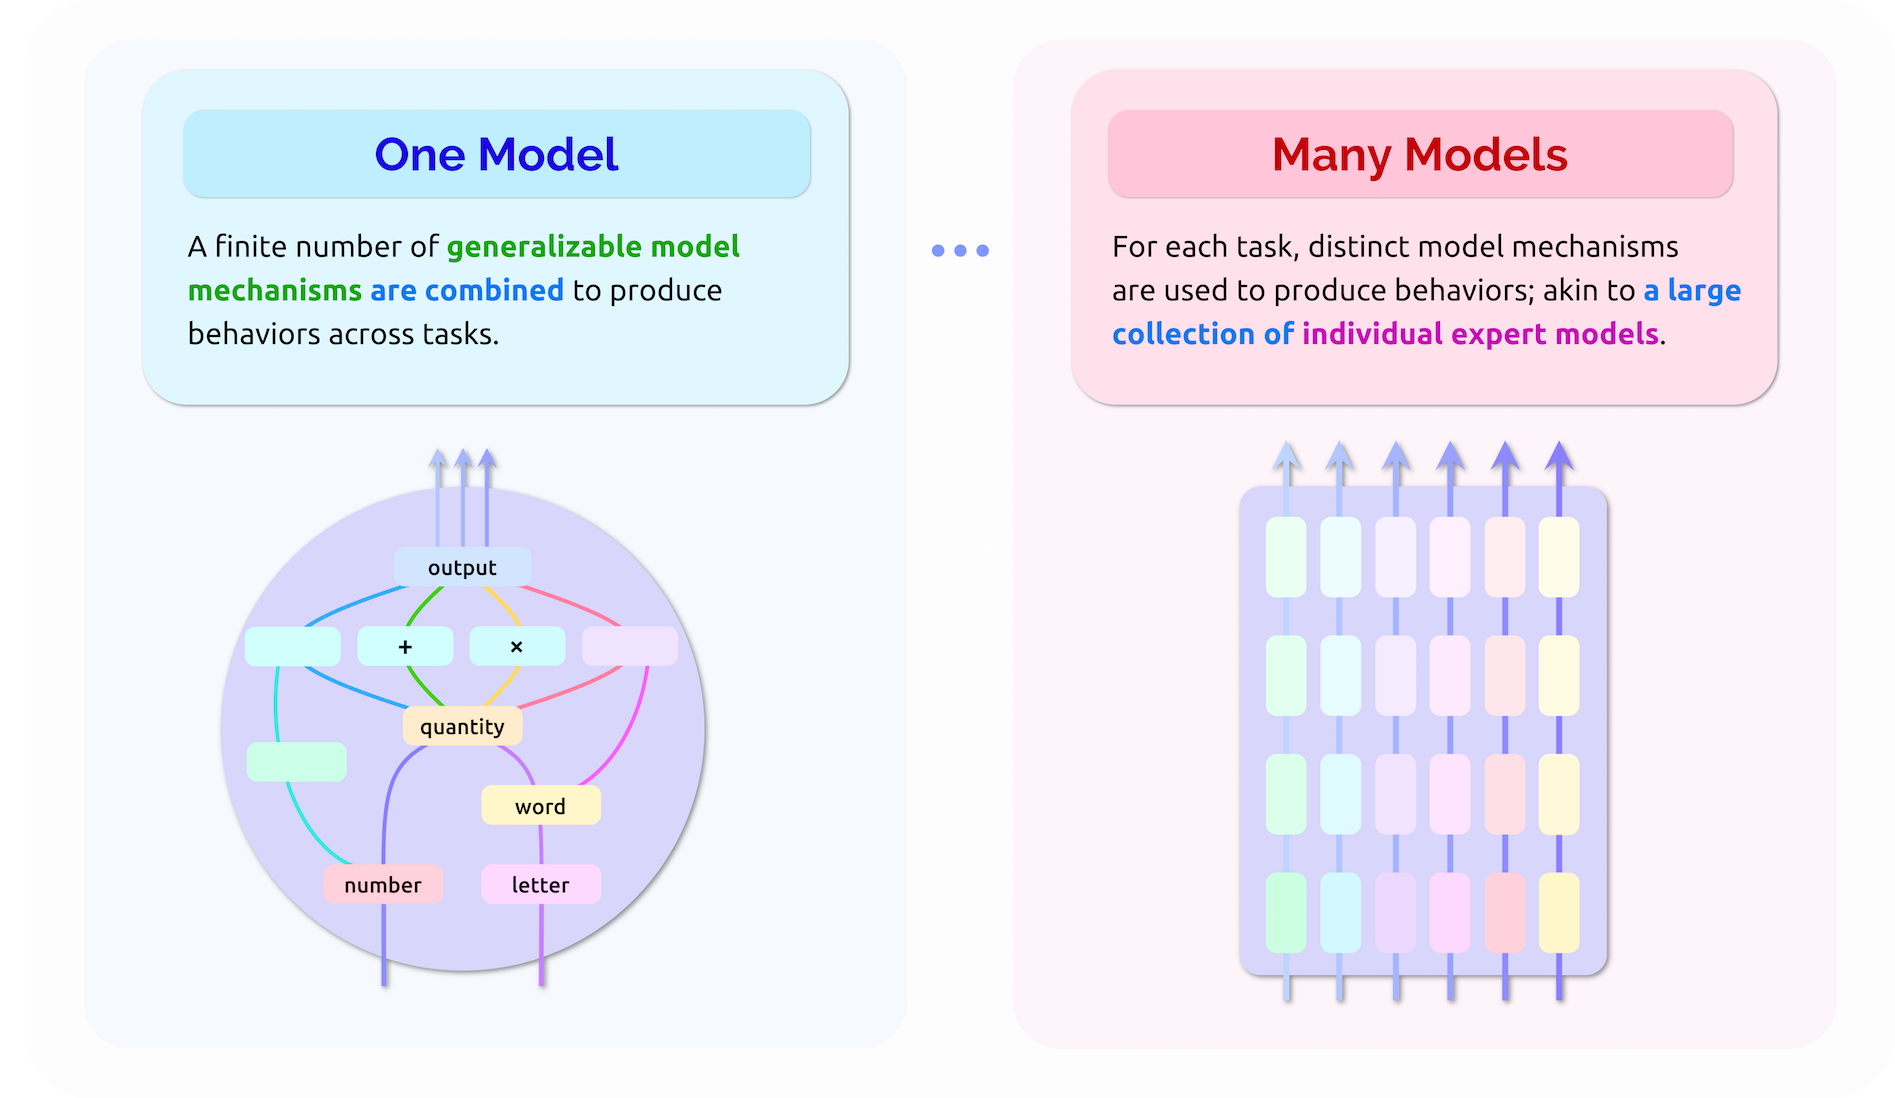
\includegraphics[width=\linewidth]{technology/figures/Interpretability.png}
    \caption{One model-many model nature of foundation models: A central question for the interpretability of a foundation model is to understand where it is located on the spectrum between \textit{one model} and \textit{many models}. As one model, behavior can be made interpretable by identifying and characterising the finite number of generalizable model mechanisms that the model uses to produce behaviors across tasks (\eg mechanisms that assign meaning to words, compare quantities, and perform arithmetic). As many models, explanations of model behavior in one task are not necessarily informative about behavior in other tasks; thus requiring to study behavior independently in each task.}
    \label{fig:intrp}
\end{figure}


\subsubsection{Characterizing behavior}
\label{sec:interpretability-behavior}

The simplest understanding of a technology is widely taken to be knowing \textit{what} does the technology do?
This seemingly straightforward question is significantly challenging for foundation models, due to the myriad of unforeseen behaviors and tasks that these models are capable of performing. 

Task-specific neural network models are trained to perform a single task in a single domain, \eg~image classification.
Their task and the input and output domains are therefore clear; yet even for these models it can be challenging to know exactly what the model will do, given a particular input: for instance, model behaviors can unexpectedly differ greatly for two perceptually similar inputs~\citep{garg2020bae,jin2020bert} or two subpopulations of the same data (stratified, for example, by race or gender~\citep{hovy2015,blodgett2016,tatman2017,buolamwini2018gender}).

This challenge of characterizing a model's behavior is amplified manyfold for foundation models.
The space of tasks that the model is able to perform is generally large and unknown, the input and output domains are often high-dimensional and vast (\eg language or vision), and the models are less restricted to domain-specific behaviors or failure modes.
Consider, for example, the surprising ability of GPT-3 to be trained on large language corpora and to subsequently develop the ability to generate mostly-functional snippets of computer programs. 
A key challenge for characterizing the behavior of foundation models is therefore to identify the capabilities that it has.
Even further, for each task that a foundation model can perform, and there may be many or infinitely many, all the challenges remain that one faces when trying to understand the behavior of much simpler, task-specific models.

Characterizing each `task' that a foundation model can perform is further complicated by their one model-many models nature (see \reffig{intrp}).
Again taking GPT-3 as an example, it was shown that it can be tailored to many tasks through simple prompting (see \refsec{adaptation}).
Yet, each task can be specified through many possible prompts and slight variations in prompts can result in meaningful changes of model behavior.
For instance, the task of sentiment classification of a movie review can be specified by presenting the movie review followed by `Her sentiment towards the film was...' or `My overall feeling was that the movie was...'; despite these prompts appearing to pose closely related tasks, GPT-3 will exhibit different response accuracies for each prompt~\citep{Zhao2021calibrate}.
Observations like these raise important questions regarding the relationship between the characteristics of prompts and the resulting model behaviors.
Specifically, can meaningfully different responses to seemingly similar prompts actually be considered as resulting from the same model or do they result from highly distinct model mechanisms, and does characterizing the behaviors of the foundation model (or its adapted derivatives) in one task truly aid in characterizing the behaviors of other possible adaptations of the model?

To identify the capabilities that a foundation model has and those it is missing, researchers can utilize controlled  evaluations.
Here, domain experts design prompts that are known to require a particular competence and then study the ability of a model to respond correctly to these prompts ~\citep{papadimitriou2020learning,DBLP:journals/corr/abs-2103-05247,kataoka2020pre,wu2021identifying,xie2021innout,koh2021wilds}.
For example, psycholinguists have designed prompts that require a language model to choose between a grammatically correct sentence and the same sentence with a specific  grammatical inaccuracy; knowing whether the model consistently prefers the grammatically correct sentence over its grammatically incorrect counterpart tells us whether the model has the particular grammatical competence required to identify this inaccuracy~\citep{linzen2016assessing}.

Given the huge range of possible capabilities of foundation models, and our current lack of any general method for determining a priori whether a foundation model will have a given capability, bespoke evaluations like these are crucial.
They allow exploring the range of behaviors that foundation models are capable of, while requiring relatively minimal model access: we only need to present inputs and receive model outputs, and we need not depend on access to the implementation or parameters of a model.
Given the infinitely many desirable and undesirable tasks, subtasks, and behaviors that foundation models may be capable of (or incapable of), characterizing model behaviors and capabilities will be increasingly challenging and important.
We believe that instead of relying on few experts to formulate and test for possible behaviors, it will be critical to extend these types of analyses to test for many more behaviors, in part by opening up this line of exploration to diverse communities and experts in many disciplines, as well as by increasing access to and scale of these evaluations.


\subsubsection{Explaining behavior}

In addition to characterizing what a foundation model is doing, one can try to characterize \textit{why} it performs certain behaviors by providing explanations of these behaviors in terms of potential causes in the data.
While current explanation approaches, which provide such explanations of behavior, can reveal qualities of inputs that affect a model's responses, they often require full access to the model to do so and are generally limited in their ability to elucidate any general model mechanisms, which foundation models use to respond to many inputs, tasks, and domains.

Current explanatory approaches can generally be understood as distinct models, which are designed to provide an explanation of particular behaviors of another \textit{black box} model. 
Importantly, these approaches are separate from the model whose behavior is analyzed, which by itself is not interpretable.
This separation can be problematic, as the provided explanations can lack faithfulness~\citep{jacovi2020towards}, by being unreliable and misleading about the causes of a behavior~\citep[c.f.,][]{rudin2019stop}.
Even further, unsound explanations can entice humans into trusting unsound models more than they otherwise would (for a detailed discussion of trust in artificial intelligence, see~\citet{jacovi2021formalizing}).
These types of concerns grow as we transition from task-specific models towards the wide adoption of foundation models, as their behavior is vastly more complex.

Current explanatory approaches can largely be divided into either providing \textit{local} or \textit{global} explanations of model behavior~\citep{doshi2017towards}.
Local explanations seek to explain a model's response to a specific input (\eg by attributing a relevance to each input feature for the behavior or by identifying the training samples most relevant for the behavior;~\citep{simonyan2013deep,bach2015pixel,sundararajan2017axiomatic,shrikumar2017learning,springenberg2014striving,zeiler2014visualizing,lundberg2017unified,zintgraf2017visualizing,Fong_2017_ICCV,koh2017understanding}). Global explanations, in contrast, are not tied to a specific input and instead aim to uncover qualities of the data at large that affect model behaviors (\eg by synthesizing the input that the model associates most strongly with a behavior;~\citep{simonyan2013deep,nguyen2016synthesizing}). 

Local and global explanations have provided useful insights into the behavior of task-specific models~\citep[\eg][]{li2015visualizing,wang2015visual,lapuschkin2019unmasking,thomas2019analyzing,poplin2018prediction}.
Here, the resulting explanations are often taken to be a heuristic of the model mechanisms that gave rise to a behavior; for example, seeing that an explanation attributes high importance to horizontal lines when the model reads a handwritten digit `7' easily creates the impression that horizontal lines are a generally important feature that the model uses to identify all sevens or perhaps to distinguish all digits.

Given the one model-many models nature of foundation models (see \reffig{intrp}), however, we should be careful not to jump from specific explanations of a behavior to general assumptions about the model's behavior.
While current explanatory approaches may shed light on specific behaviors, for example, by identifying aspects of the data that strongly effected these behaviors, the resulting explanations do not necessarily provide insights into the model's behaviors for other (even seemingly similar) inputs, let alone other tasks and domains.

%It is tempting to sidestep these types of post-hoc explanations all-together by leveraging the generative abilities of foundation models in the form of self-explanations.
%That is, we may be inclined to train foundation models to generate not only the response to an input, but to jointly generate a human-understandable explanation of that response.
Another approach could be to sidestep these types of post-hoc explanations all-together by leveraging the generative abilities of foundation models in the form of self-explanations~\citep[c.f.,][]{elton2020self,chen2018looks}.
That is, by training these models to generate not only the response to an input, but to jointly generate a human-understandable explanation of that response.
While it is currently unclear whether this approach will be fruitful in the future, there are reasons to be skeptical: language models, and now foundation models, are exceptional at producing fluent, seemingly plausible content without any grounding in truth.
%Simple self-generated “explanations” are likely to follow suit.
Simple self-generated “explanations” could follow suit.
%We need to be discerning of the difference between creating plausible-sounding explanations and gaining true insights into model behavior; even humans are famously bad at explaining their behavior~\citep[\eg][]{miller1985egotism,shepperd2008exploring}.
It is thus important to be discerning of the difference between the ability of a model to create plausible-sounding explanations and providing true insights into its behavior.



\subsubsection{Characterizing model mechanisms}

Deep understanding of systems is generally taken to mean understanding \textit{how} a system performs: which knowledge and mechanisms does it contain, and how are these assembled to form the whole?

If this is indeed possible, characterizing the representations within foundation models and the mechanisms that operate on them will be central to satisfying the desire to thoroughly understand these proliferating models; and whether these mechanisms are many and specific or few and generalizable (see \reffig{intrp}), they are at the core of the ability of foundation models to adopt a wide range of behaviors in varied tasks and domains.

To make the notions of model representations and mechanisms concrete, consider a simple behavior exhibited by GPT-3: 
It was quickly observed \textit{what} GPT-3 did when provided with examples of the addition of small numbers and then queried to perform addition of two new numbers; with high probability, it predicted the correct result of the addition~\citep{branwen2020gpt,brockman2020math}.
When asking \textit{why} GPT-3 performed as it did, one could find evidence in the input, like aspects of its prompt that highly affected its response (these might be the two numbers to be added, though not necessarily), or aspects of GPT-3’s training data that affected its response (these might be examples of addition, though not necessarily).
Delving into the model, we may envision a deeper understanding of the mechanisms that GPT-3 uses to add a specific pair of numbers and the mechanism that it uses to add other arbitrary pairs of numbers.
We may also envision a deeper understanding of whether these mechanisms are similar to the mathematical notion of 'addition' or merely correlated with this notion.

By understanding individual model mechanisms, we can build up a compositional understanding of complex behaviors of a foundation model.
A task slightly more complex than the addition of numbers is solving mathematical word problems, in which numbers come with units and the problem is presented in natural language. 
Once we understand the mechanism (or mechanisms) by which a model performs addition, we can investigate whether this mechanism is used as an intermediate step in solving the word problems.
If the addition mechanism is used, we have built up our understanding of how the model solves word problems, we have increased confidence that the foundation model generalizes the notions of quantities and addition (not another correlation or heuristic), and, furthermore, we have increased confidence in our ability to predict the model's \textit{why} (which parts of the inputs it is attending to) and the output's \textit{what} (addition of two numbers).
If the addition mechanism is not used, we may retain a healthy skepticism that this is truly addition, and we can investigate which representations and mechanisms are used instead.

It is important to be aware that there are many potential cases of more complex and concerning model mechanisms, for instance, the estimation of race from the characters in a name, or the pixels in an image.
Establishing evidence of such a mechanism in a foundation model and its use can support a moral or legal responsibility to ban the model from tasks like predictive policing, marketing, loan applications, and surveillance at large.

A plethora of methods have emerged to investigate these internal aspects of neural network models. Typically, these approaches separate the model into nodes (\eg neurons, layers, or parts of layers), then interrogate either the representations captured in nodes or the mechanisms by which nodes are assembled. 
Some approaches are hypothesis driven: by hypothesizing that nodes may capture certain information (\eg a grammatical feature of a word, or the race of a person), one can probe all nodes to quantify how much of that information they make available \citep{alain2016understanding,veldhoen2016diagnostic,belinkov2017what,adi2017finegrained,conneau2018what,hewitt2019control,hewitt2019structural,voita2020informationtheoretic,pimentel2020information}. 
Other approaches build on explanatory methods, and, instead of identifying which data cause a certain behavior, they seek to identify which data cause a certain node to activate, or which nodes cause another node later in the model to activate, thereby uncovering collections of model representations and mechanisms
%(\eg there is evidence that wheel-detecting nodes and door-detecting nodes are assembled to form car-detecting nodes)
~\citep{olah2020zoom,mu2020compositional,carter2019activation,goh2021multimodal}.
Taken together, these approaches inspect the interior of models and provide a %conceptual and concrete
basis for the ongoing explorations of the behavior of foundation models. 
Yet, the number of potential representations and mechanisms within foundation models is vast, particularly given their one model-many models nature (see \reffig{intrp}), and these types of approaches often only capture a small slice of a model's interiority.
It is thus an open challenge to expand the discovery of representations and mechanisms and to elucidate those that are most relevant or general for model behavior.
As with many approaches to interpreting foundation models, these types of explorations will benefit from including and supporting more diverse and interdisciplinary investigators and from  more accessible, flexible, and scalable methods of discovery.


In summary, we believe that the one model-many models nature of foundation models (see \reffig{intrp}) provides novel opportunities and challenges for current interpretability research: there are many adaptations of a single foundation model, and we simply do not know the extent to which they share common mechanisms.
To the extent that mechanisms are shared, understanding foundation models may be a tractable problem of characterizing these mechanisms and their relations.
To the extent that mechanisms are independent, each adaptation of a foundation model must be analyzed independently, leading to profound uncertainty about the nature of any new adaptation of the foundation model.


\subsubsection{Impacts of non-interpretability and interpretability}
\label{sec:interpretability-impacts}

Lastly, we would like to highlight that the wide adoption of foundation models is at odds with a recent plea of many interdisciplinary researchers not to use complex black box models for high stakes decisions~\citep[\eg][]{rudin2019stop}, but instead to focus on the long-standing development and application of more intrinsically interpretable models. 

In the midst of these pleas, work aimed at interpreting foundation models is a double-edged sword.
Large machine learning models, and now foundation models, are often solely deployable by powerful corporations and institutions, and incremental advances in interpretability can be exaggerated to `ethics-wash' and continue use of models as though they have \textit{achieved} interpretability, belying the reality that they remain far below traditional standards of algorithmic interpretability.
Moreover, when approaches to interpretability regularly presume easy access to models and their implementation and parameters, interpretability can serve not only as cover for powerful institutions but also centralize model knowledge in the same hands.
For those working toward the interpretability of foundation models, it is a responsibility to consistently ask whether one is working toward 
making foundation models \textit{interpretable to researchers and model owners} or \textit{interpretable to everyone}. 

Simultaneously, to the extent that foundation models are already being deployed, work on interpretability presents unique opportunities to shift knowledge of foundation models, and thus power, back to datafied and evaluated peoples. 
Interpretation can facilitate the discovery of societally salient aspects of models.
More radically, work creating accessible methods that allow anyone to interpret the behavior of foundation models shifts power to diverse peoples, creating opportunities to investigate models, opportunities to discover aspects of models important to individuals or their communities, and opportunities to meaningfully consent to, improve, or all-together contest the use of foundation models.
It is also important for researchers to view the interpretability of foundation models as not only a goal, but a question: work can serve to explore and assess whether the lack of foundation model interpretability is intrinsic and should be deeply studied and widely known as a serious issue discouraging use (or increasing regulation) of these systems, or whether it is possible for future foundation models to uphold a high standard of interpretability for all. 
% It is crucial for those aiming to interpret foundation models to regularly ask \textit{To whom is this model interpretable?} and, if the answer is not aligned with societal needs, \textit{wh}

% When foundation models are deployed, the challenge and opportunity of understanding how the behaviors of foundation models emerge\dash{}from a small set of very powerful and versatile mechanisms or a wide range of highly-specialized mechanisms\dash{}enables and requires interpretability work to move its focus away from studying individual input-response associations towards identifying and understanding mechanisms essential to many foundation model responses across many inputs, tasks, and domains.



% %%%%%%%%%%%%%%%%%%%%%%%
% %%%%%%%%%%%%%%%%%%%%%%%
% %%%%%%%%%%%%%%%%%%%%%%%
% % OLD COMMENTS:
% %%%%%%%%%%%%%%%%%%%%%%%
% %%%%%%%%%%%%%%%%%%%%%%%
% %%%%%%%%%%%%%%%%%%%%%%%


% OLD introduction:
%Compared to most other machine learning models, foundation models are characterized by a vast increase in training data and complexity and the emergence of unforeseen capabilities: foundation models are able to do unforeseen tasks and do these tasks in unforeseen ways. The increasing adoption of foundation models thereby creates growing desires, demands, and unprecedented challenges for understanding their behavior.

%In contrast to task-specific models, foundation models are typically trained with a task-agnostic objective function
%across vast and highly disparate datasets, potentially spanning many domains and modalities (see \refsec{training}).
%Through this training, they learn an exceptionally wide range of behaviors, which can vary profoundly between tasks and domains, as demonstrated by their ability to be adapted to many different types of downstream tasks and to exhibit behaviors that are specific for each of these tasks (see \refsec{adaptation}).
%It is thus challenging to answer even the seemingly simplest question: \textit{what capabilities} does a foundation model  have?
%Moreover, it is an open question to what extent these diverse behaviors rely on distinct or shared \textit{model mechanisms}, akin to  algorithmic building blocks within the model.
%We argue that this question is central to understanding foundation models: while foundation models are single models with fully shared computations, they can also be understood as a large collection of mutually-informed expert models.
%In the following, we refer to this as the \emph{one model-many models} nature of foundation models.



% In this section we discuss approaches to interpreting and analyzing the behavior of neural network models, and identify where novel challenges and opportunities arise for foundation models.

% Whereas earlier models were typically trained to be capable of doing one or few intended tasks, for foundation models

% we have only uncovered a small fraction of the capability surface of foundation models.
% Delving deeper into the model, 

% , which are composed to allow for diverse behaviors.
%We argue that due to the high diversity of the behaviors that foundation models can perform, which potentially involve distinct \textit{sub-functionalities} (conceptually, distinct algorithmic building blocks) of the model, they can at the same time be understood as single models with fully shared computations and parameters, but also as a collection of distinct models specified through (sometimes minimal) adaptation, each designed to solve a specific task.

%We argue that one particular challenge for understanding foundation models is posed by the fact that a single foundation model be adapted to a multitude of downstream tasks, and thus exhibit a multitude of distinct behaviors on such tasks.
%We term this the \emph{one model-many models nature of foundation models}: while foundation models can be understood as single models with fully shared computations and parameters, they can at the same time be interpreted as a collection of mutually informed individual expert models, each designed to solve a specific task. \pw{I was a bit confused by this\dash{}do the individual expert models refer to what happens after adaptation? So ``they'' means ``the collection of all foundation models'' as opposed to ``a single foundation model''? I read through Percy's outline of the intro but didn't come across this duality, at least phrased this way.}
%\rb{Agree with Pang Wei that this abstraction, if its important, needs to be developed a bit more thoroughly and is somewhat confusing/unclear. Also not really clear to me what exactly this means; how do we get this factorization into experts, what are the assumptions/are these disjoint in some sense (and does that mean such a factorization reliably exists), or is there some kind of information bottleneck type thing going on here (\ie~you are calling the smallest subnetwork that retains performance on the task, or something in this spirit, the expert model?)?}
% \bln{\sout{By combining a generative learning mechanism with highly diverse training datasets, foundation models are not restricted to solving a set of a priori defined data problems.
% This seems like it will be covered in other sections and does not need to be stated here vvv
% Note that foundation models are distinct from multi-task models, which are trained to solve a predefined set of tasks in a limited number of domains~\citep{ruder2017overview}. 
%Instead, foundation models can be conceptualized as a highly versatile clay out of which other models, specialized for distinct tasks and domains, can be formed. 
%Can probably cut these few sentences because this info will be covered in the intro.
% A key challenge is characterizing model mechanisms, while also contending with uncertainty surrounding whether understanding model mechanisms in one task is informative about the model's behavior in other tasks or domains.
% , which enable them to build these individual expert models and that can generalize knowledge across domains.
% In addition, researchers studying the behavior of foundation models will be faced with challenges arising from the one model-many models nature of these models, as it is unclear to which degree knowledge about their behavior in one task is informative about behavior in other tasks or domains.

% Towards systematizing this area of study, we structure our discussion according to three levels at which the behavior of neural network models can be analyzed~\citep[inspired by][]{marr1982vision}:
%will take inspiration from Marr’s levels of analysis~\citep{marr1982vision} to discuss how one can understand the behavior of foundation models, and other neural network models in general.
%In particular, we will ask three questions:

% Put simply, we will first discuss how one can characterize \textit{what} a neural network model is doing, then \textit{why} it is doing it, and lastly \textit{how} it does it.

% — arguably the most speculative and difficult question to answer.

% , expanding upon positive and negative potential consequences.
% \color{purple}{[Ria: We may want to reference that after describing the key opportunities and challenges in foundation model interpretability, we will return to some of the most clear societal implications.]} \color{black}

% given an input, what does the technology do?The foundation for understanding any complex model is to characterize \textit{what} it does by characterizing its behavior across its possible inputs.

% Prior work shows that characterizing the behavior of task-specific neural networks, which are trained to perform a single task (e.g.~object classification) in a specific domain, is challenging.

% Thus, despite a network potentially boasting high predictive accuracies, coming to an interpretable definition of when one can be confident the network will work well in practice is quite difficult. 
% Even if a task-specific model boasts high average predictive accuracy, it can be challenging to fully characterize the behaviors that the model will exhibit across the possible inputs of a task.
%\rb{This sentence doesn't really make much sense to me/not sure what is the rhetorical intent or why it follows the previous one. \ie~you say it is hard to characterize and then characterize the behavior, so if anything that seems to show the opposite. I could see saying something like \textit{because the models don't behave systematically, and this makes them hypersensitive, it is hard to make valid assumption on their behavior} but not sure why we are getting stuff like subpopulation performance or fairness considerations here/what you want the reader to takeaway}.

% foundation models are distinct in that they are trained with a general objective function on diverse data, not on a specific task in a specific domain (see \refsec{training}).

% Thus, in addition to characterizing how the model behaves on different inputs for a task, foundation models pose the question of identifying which types of tasks are feasible for this model.

%Concretely, one does not have to work hard to ask of an image classifier, \textit{is this system capable of generating labels that classify between dog and cat, perhaps inaccurately?}, as one can simply see if \textit{dog} and \textit{cat} are in its finitely many human-specified labels \pw{I think people might object to this: just because dog and cat are in the label set, and in fact, just because it might get high accuracy on dogs and cats in some test set, doesn't mean that it can classify between dog and cat in the sense that it knows how to really do the classification} \rb{Do you even need this preamble? I think you can take as read that the reader has read the intro/has a sense of what a foundation model is? It seems like the point you want to make is the set of plausible or potential behaviors is somewhat unbounded for foundation models (and I guess is fully specified for an image classifier with a specific fixed label space), which is a great point, but I don't know if you really need this setup as it seems like you can get to the punchline pretty quickly/it is not a terribly unintuitive point.}; likewise, one would not ask of the same image classifier, \textit{can this summarize news articles?}, as the answer \textit{no} is apparent.
%For foundation models, even these seemingly \bln{\sout{trivial} simple} questions are \bln{\sout{uncertain} difficult to answer} before careful study; a given foundation model very well might be able to summarize news articles and classify between dogs and cats. \bln{Seems like there are two components of understanding behavior in this paragraph: 1) what the model does (eg given an image of a cat, what label does a model assign?) and 2) what tasks the model \textit{can} perform (eg does the model's output space include ``cat'' and ``dog''). Maybe these should be more clearly distinguished? (or maybe the universality of foundation models implies that 2 is ``all tasks'' and doesn't have to be discussed here?)}% My intuition is that the first is more important for ``characterizing behavior'' as} 

% The one model-many models nature of foundation models adds another level of difficulty to characterizing model capabilities.
% Understanding foundation models as a collection of distinct interpretable tasks is itself a simplification complicated by their one model-many models nature.

%Taking GPT-3~\citep{brown2020language} as a concrete example, it has been shown that by partially specifying the input to GPT-3 as a \textit{description of the task to be performed}, the behavior of GPT-3 can be tailored to a wide variety of tasks \bln{Maybe can point to adaptation section rather than re-explain prompting?}.
% This is demonstrated by the two sentiment classification prompts below, each of which contains a guiding example and a query:
% \begin{quote}
% Prompt 1: \\
% \textit{Here is what our critics think for this month’s films.\\
% One of our critics wrote ``This movie is amazing!''. Her sentiment towards the film was positive.\\
% One of our critics wrote ``Horrific movie, don’t see it''. Her sentiment towards the film was ...}\\
% Prompt 2: \\
% \textit{This movie is amazing! My overall feeling was that the movie was good.\\
% Horrific movie, don’t see it. My overall feeling was that the movie was ...}
% \end{quote}

% the relationships between the way a task is specified and the resulting adapted model, 
%\pw{Oh, I had misunderstood the single model\dash{}many model duality. I guess you mean that the same model can be interpreted as having multiple models? In general, I'm a bit confused by what this duality means.} \rb{1) Agree with Pang Wei that the whole duality thing is confusing me, and I am not clear if I am not following properly or you are using the duality in a slightly different way than defined and 2) This is a very extensive point, that is somewhat language-centric, and seems to amount to \textit{the behavior of the foundation model \{actually I would hesitate to say the foundation model, I think we are viewing prompting-based methods as adaptation methods\} is dependent on the adaptation mechanism}; do we need this extended example to make that clear?}

%Based on these challenges, we now proceed to discuss potential avenues for future research to characterize the behavior of foundation models.

% (inspired by xxxcite ex in CV and xxxcite ex in NLP).
% , as recently done in computer vision (CV) and natural language processing (NLP).
%\rb{I would recommend changing this framing. Similar to other sections, I might detail the current status quo for behavioral analysis with citations, and then talk about the fundamental questions/desiderata for interpretabilty and so on, \ie~do more framing/conceptual work of asking richer questions and setting the stage, and perhaps mention what paradigms that already exist and promisng and what doesn't, but avoid claiming specific solutions will work best. I think deeper stage-setting and framing will have both more utility and longevity; figuring out which path will work can be done in subsequent standard concrete research rather than requiring speculation that may easily prove long/lack longevity.}

%relatively small datasets \rb{Why does this matter? This seems like a property of the current paradigm, surely isn't the desiderata (I could imagine saying something like controlled or precisely designed or so on)/seems more incidental?} of

% who are able to formulate contextually important behaviors. 
%one simply needs to be able to provide \bln{\sout{(a large number of)}} inputs to the foundation model and collect its responses.
%\rb{It seems like the important points are a) the involvement of domain experts who understand complex phenomena deeply in evaluation design and b) potentially disucssion of the relationship between humans and foundation models, though not super convinced this generally makes sense (e.g.~foundation models for proteins clearly don't do anything akin to humans, since notably humans are not doing protein folding). Regardless, I would emphasize these points and put the psycholinguists point as perhaps a paranthetical example rather than the other way around.}
% By having experts in different domains craft such evaluations, we can begin to understand to what extent the foundation model is subject to the one model-many models duality.
%\pw{Might be worth trying to sync up with the people writing the Evaluation section? This whole subsection seems like it could arguably belong there (since presumably we want to be able to evaluate what foundation models can do); and at least, the preceding two paragraphs center around how we should evaluate foundation models. But I think the current Evaluation outline doesn't mention any of this sort of evaluation.} \rb{Agreed, we should figure out the balance. I would actually say stick with this split, \ie discussion both representational and behavior analysis under interpretability since there will be synergies, and let evaluation focus on downstream things and adaptation and so on}

% \color{purple}{Ria: I think in several pieces of the Inerpretability section, it's important to note that assuming that we the experts can come up with every possible interesting hypothesis and test it was being stretched to its limits in normal neural nets and in order to avoid being short-sighted we should expect going beyond this incremental approach as a critical future research direction!}\color{black}

% In contrast, global explanations are not tied to a specific input and instead aim to uncover the more general characteristics of the association between data and model responses (\eg by identifying or synthesizing the input that the model associates most strongly with a behavior;~\citep{koh2017understanding,simonyan2013deep,nguyen2016synthesizing}.

% vvv I think this belabors the point vvv
% To take a concrete example in NLP, methods from psycholinguistics have been used to create controlled evaluations that test the grammatical competence of neural language models.
% Consider the following pair of sentences, one grammatical, and one ungrammatical (marked with an asterisk [*]):
% \begin{quote}
% 	*The keys to the cabinet by the door is on the table.	(1)\\
% 	The keys to the cabinet by the door are on the table.	(2)
% \end{quote}
% In English, main verbs must agree with their subject in number; 
% by evaluating whether a neural language model prefers sentences like (2) over sentences like (1), psycholinguists can carefully test whether the behavior of a neural network is consistent with human understanding of syntax.

% knowing the importance of certain features of the data for specific model behaviors does not necessarily provide  insights into the model mechanisms activated by purportedly similar inputs, let alone other inputs, tasks, and domains.
% vvvv Ria: I like this line, but I don't know what it means. If whoever wrote it wants to include it, it would be helpful to me to hear more about what it means!
% other domains, as these might be distinct, too many, and too diverse.
% Instead, we argue that a central component to understanding foundation models will be to understand how they are able to quickly generalize knowledge across tasks and domains, as demonstrated by their ability to be easily adapted to a multitude of downstream tasks in different domains (see \refsec{adaptation}) by the use of few training samples or in-context learning~\citep{brown2020gpt3}. 
% While current explanatory approaches might 
% % help improve the interpretability of 
% shed light 
% foundation models in very specific tasks and domains, by relating their responses to the characteristics of the data, they seem highly limited in their ability to identify any fundamental, more general patterns of the association between input and response that foundation models might exhibit across different downstream tasks or domains.
% Identifying these patterns is essential, however, to 

% understanding the mechanisms, which enable the generalization of knowledge and which separate foundation models from other neural network models.

%In addition, the one model-many model nature of foundation models makes it more difficult to gain insights from explanation studies. Concretely, foundation models add the challenge of disentangling \textit{importance for the type of behavior (or task) that the foundation model performs} (\eg sentiment analysis), from \textit{importance for the specific behavior that it performs} (\eg positive or negative). The former type of importance is not a confounding factor in single-purpose or multi-task models, and so, current explainability are not aimed at disentangle the two. \bln{I'm not quite sure I follow the distinction here. If something is important for sentiment analysis doesn't that mean it is important for predicting a positive or negative sentiment?} \pw{I'm also a bit lost here. I just read the healthcare section so I'm thinking about those applications. Say we have a foundation model that's trained on text and images, and then adapted for an x-ray diagnosis task. How do I map the single model\dash{}multi-model duality onto this application? Or is that just specific to text? It seems pretty reasonable to still try to explain x-ray diagnoses through the usual methods?}

% While it is unclear whether this approach could be fruitful, there are reasons to be skeptical: foundation models, and the language models that preceded them, are exceptional at producing fluent, plausible-sounding content, but without any grounding.

% Deep understanding the behaviour of neural network model requires understanding \textit{how} the model performs a task: what concepts is it learning, and how are they used?
%While inextricably linked to understanding why the model performs a certain way (see the previous section), this question focuses not on explaining individual model responses by relating them to the features of the input, but rather centers on characterizing the internal model mechanisms giving rise to these responses.

% the sorts of representations and mechanisms we are interested in uncovering, and to present the emerging approaches to uncovering them, consider the following examples:

% but instead of attributing a \textit{model behavior} to particular data, they attribute a \textit{node's behavior} to certain data, or attribute a node's behavior to earlier nodes' behavior, uncovering a collection of representations and mechanisms (xxxcite building blocks, circuit, attention).

%  and take it through the three described levels of analysis.
% To make this concrete, let’s take a simple behavior exhibited by GPT-3. %  and take it through the three described levels of analysis.

% A more reliable and deeper explanation, however, would describe the mechanism that GPT-3 uses to add arbitrary numbers; this is the \textit{how}.
%Understanding general mechanisms is crucial because they may or may not play a role in more complex tasks, like solving simple natural language mathematics problems. 
%We might call the ability to add numbers a \textit{mechanism} of the foundation model that could also play a role in more complex tasks, like solving simple natural language mathematics problems. 

% we can characterize how the model solves these word problems, confident that will be able to solve the mathematics word problems in generality, and immediately have insight into how.
% If the addition mechanism is used, we can have increased confidence that the foundation model is relying on true addition, not a correlation or heuristic, and will be able to solve the mathematics word problems in generality, and immediately have insight into how.

% If the addition mechanism is not used, then we may investigate start from scratch in understanding how the foundation model attempts to solve the task.
% Understanding what mechanisms exist in the foundation model is a step towards understanding how more complex tasks are performed by the foundation model.
% In the example of addition, a slightly more complex task might be solving mathematical word problems, in which numbers come with units and the problem is presented in natural language. 
% % (\eg ``If I had 5 melons and were given 3 more, how many melons would I have?'')
% If we understand the mechanism by which addition is performed by the model, we can then ask if this mechanism is used as an intermediate step in solving the mathematics problems.
% If the addition mechanism is used, we can have increased confidence that the foundation model will be able to solve the mathematics problems in generality, and immediately have insight into how.
% If the addition mechanism is not used, then we must start from scratch in understanding how the foundation model attempts to solve the task.

% The one model-many models nature of foundation models will challenge researchers to move beyond their own hypotheses and the sheer magnitude of representations and mechanisms  
% Characterizing such a mechanism, and determining the extent to which it is used by the foundation model, could provide strong evidence against the use of \textit{any} adaptation of foundation models; for example in tasks such as predictive policing, loan application evaluation or shoplifting risk detection.
%The characterization of this subfunctionality would help in detecting

%The results of intermediate computations, like the addition of 5 and 3 in processing the sentence ``If I had 5 melons and were given 3 more, how many melons would I have?'' could result from such an addition subfunctionality. \bln{Having the word problem in the middle of the sentence reads awkwardly.}
%The composition of subfunctionalities\dash{}solving simple problems independently and then combining their solutions in generality to solve more complex problems\dash{}is a desirable property in AI systems.
%This brings the one model-many models duality of foundation models to the fore\dash{}to what extent are simple subfunctionalities being combined to allow for a wide range of behaviors, versus a large set of independent behaviors being memorized through brute force? \pw{Is this specific to foundation models? For example, people often say that CNNs first do edge detection, then higher layers maybe try to recognize parts, etc.?}

% the extent to which non-interpretable and mildly interpretable models prevent datafied and evaluated from meaningfully consenting, protecting themselves, or investigating and contesting the use of foundation models.

% It is important to discern the
% % the jarring, 
% % often unstated 
% difference between work making foundation models \textit{interpretable  to researchers and model owners} and visions of making foundation models \textit{interpretable to everyone}. 





% %%%%%%%%%%%%%%%%%%%%%%%
% %%%%%%%%%%%%%%%%%%%%%%%
% %%%%%%%%%%%%%%%%%%%%%%%
% % OLD VERSION:
% %%%%%%%%%%%%%%%%%%%%%%%
% %%%%%%%%%%%%%%%%%%%%%%%
% %%%%%%%%%%%%%%%%%%%%%%%


% % \subsection{Interpretability}
% % \label{sec:interpretability}

% % \status{in progress}

% % %\begin{figure}[ht]
% % %\centering
% % %\includegraphics[scale=0.3]{example-image-a}
% % %\caption{\label{fig:interpretability} \todo{explain}}
% % %\end{figure}
% % %
% % %As \reffig{interpretability} shows, we know nothing.

% % The wide adoption of foundation models will lead to an increase in stakeholders interested in understanding their behavior as well as novel methodological challenges for explaining this behavior.
% % In this section we discuss approaches to interpreting and analyzing the behavior of neural network models, and identify where novel challenges and opportunities arise for foundation models.

% % foundation models are trained with general objectives across highly diverse datasets, potentially spanning many domains and modalities (see \refsec{training}.
% % Due to this diversity, they adapt an extremely wide range of possible behaviors, as demonstrated by their ability to be easily adapted to a multitude of downstream tasks, and to exhibit a multitude of distinct behaviors on such tasks (see \refsec{adaptation}).
% % We argue that these diverse behaviors potentially involve distinct \textit{sub-functionalities} (conceptually, distinct algorithmic building blocks) of the model and that while foundation models represent single models with fully shared computations, they can therefore also be understood as a collection of individual mutually-informed expert models.
% % This raises the question to which degree knowledge about model behavior in one task and domain is informative about the model's behavior in another task or domain.
% % %We argue that due to the high diversity of the behaviors that foundation models can perform, which potentially involve distinct \textit{sub-functionalities} (conceptually, distinct algorithmic building blocks) of the model, they can at the same time be understood as single models with fully shared computations and parameters, but also as a collection of distinct models specified through (sometimes minimal) adaptation, each designed to solve a specific task.
% % In the following, we will refer to this as the \emph{one model-many models nature of foundation models}.
% % %We argue that one particular challenge for understanding foundation models is posed by the fact that a single foundation model be adapted to a multitude of downstream tasks, and thus exhibit a multitude of distinct behaviors on such tasks.
% % %We term this the \emph{one model-many models nature of foundation models}: while foundation models can be understood as single models with fully shared computations and parameters, they can at the same time be interpreted as a collection of mutually informed individual expert models, each designed to solve a specific task. \pw{I was a bit confused by this\dash{}do the individual expert models refer to what happens after adaptation? So ``they'' means ``the collection of all foundation models'' as opposed to ``a single foundation model''? I read through Percy's outline of the intro but didn't come across this duality, at least phrased this way.}
% % %\rb{Agree with Pang Wei that this abstraction, if its important, needs to be developed a bit more thoroughly and is somewhat confusing/unclear. Also not really clear to me what exactly this means; how do we get this factorization into experts, what are the assumptions/are these disjoint in some sense (and does that mean such a factorization reliably exists), or is there some kind of information bottleneck type thing going on here (\ie~you are calling the smallest subnetwork that retains performance on the task, or something in this spirit, the expert model?)?}
% % % \bln{\sout{By combining a generative learning mechanism with highly diverse training datasets, foundation models are not restricted to solving a set of a priori defined data problems.
% % Note that foundation models are distinct from multi-task models, which are trained to solve a predefined set of tasks in a limited number of domains~\citep{ruder2017overview}.
% % %Instead, foundation models can be conceptualized as a highly versatile clay out of which other models, specialized for distinct tasks and domains, can be formed. 
% % %Can probably cut these few sentences because this info will be covered in the intro.
% % A key challenge for understanding the behavior of foundation models is to identify the universal representations that enable them to build these individual expert models and that can generalize knowledge across domains. 

% % Towards systematizing this area of study, we will structure our discussion according to three levels at which neural network models can be studied~\citep[inspired by][]{marr1982vision}:
% % %will take inspiration from Marr’s levels of analysis~\citep{marr1982vision} to discuss how one can understand the behavior of foundation models, and other neural network models in general.
% % %In particular, we will ask three questions: 
% % First, we will discuss how one can characterize \textit{what} a neural network model is doing, then \textit{why} it is doing it, and lastly \textit{how} it does it.
% % For generally any model, the three questions become increasingly more challenging to answer.
% % Intuitively, the question of \emph{what} concerns characterizing the model's outward behavior without ``peeking inside."
% % The increasingly more challenging question of \emph{why} concerns providing explanations of a specific behavior in terms of potential causes in the data.
% % %, which requires examining how the model interacts with data more closely.
% % Finally, the question of \emph{how} dives into understanding the internal mechanisms that drive how the model performs a task, which is arguably the most speculative, and most difficult to satisfy.
% % The next three sections will each address each of these questions as they concern foundation models.

% % \subsubsection{Characterizing behavior}
% % The foundation for understanding any complex model is to characterize \textit{what} it does: to characterize its behavior across its possible inputs.
% % We argue that this seemingly straightforward question will be uniquely challenging for foundation models, due to the diversity of distinct types of behavior (or tasks) that they may be able to perform. % \rb{Can we simplify to \textit{The generative capabilities of foundation models make this uniquely challenging}? Also agree with Pang Wei's subsequent comment which supersedes this.}. 
% % %\pw{Reading the rest of this section, I wasn't very sure why the generative part was the important bit, since we talk about task-agnosticity and adaptation later; is the claim that generation is necessary for those things?)}

% % Prior work shows that characterizing the behavior of task-specific neural networks, trained to perform a single task (e.g.~object classification), is challenging.
% % Their behavior can, for example, differ greatly for two perceptually similar inputs (xxxcite) and different subpopulations of a dataset (stratified, for example, by race or gender;~\citep{hovy2015,blodgett2016,tatman2017}).
% % Thus, despite a network at first sight boasting high predictive performance, coming to an interpretable definition of when one can be confident the network will work well in practice is quite difficult. \athms{maybe instead: Thus, even if a network boasts high predictive accuracies, it can be challenging to fully characterize the behaviors that the model will exhibit across its possible inputs.}

% % %\rb{This sentence doesn't really make much sense to me/not sure what is the rhetorical intent or why it follows the previous one. \ie~you say it is hard to characterize and then characterize the behavior, so if anything that seems to show the opposite. I could see saying something like \textit{because the models don't behave systematically, and this makes them hypersensitive, it is hard to make valid assumption on their behavior} but not sure why we are getting stuff like subpopulation performance or fairness considerations here/what you want the reader to takeaway}.
% % \athms{This is even more challenging for foundation models.} foundation models are distinct in that they are trained with a general objective function on diverse data, not on a specific task for a specific domain (see \refsec{training}).
% % They are thus much less restricted to certain domain-specific behaviors when compared to other neural network models.
% % Concretely, foundation models open up a wide new range of questions relating to what \textit{types} of behaviors they can (approximately) perform, such as the surprising ability of GPT-3 to generate mostly-functional code snippets.
% % Thus, in addition to the ``how does this model behave on different categories of inputs for this task'' questions that arise in analyzing single- and multi-task models, foundation models require asking ``what tasks are feasible for this model?''

% % %Concretely, one does not have to work hard to ask of an image classifier, \textit{is this system capable of generating labels that classify between dog and cat, perhaps inaccurately?}, as one can simply see if \textit{dog} and \textit{cat} are in its finitely many human-specified labels \pw{I think people might object to this: just because dog and cat are in the label set, and in fact, just because it might get high accuracy on dogs and cats in some test set, doesn't mean that it can classify between dog and cat in the sense that it knows how to really do the classification} \rb{Do you even need this preamble? I think you can take as read that the reader has read the intro/has a sense of what a foundation model is? It seems like the point you want to make is the set of plausible or potential behaviors is somewhat unbounded for foundation models (and I guess is fully specified for an image classifier with a specific fixed label space), which is a great point, but I don't know if you really need this setup as it seems like you can get to the punchline pretty quickly/it is not a terribly unintuitive point.}; likewise, one would not ask of the same image classifier, \textit{can this summarize news articles?}, as the answer \textit{no} is apparent.
% % %For foundation models, even these seemingly \bln{\sout{trivial} simple} questions are \bln{\sout{uncertain} difficult to answer} before careful study; a given foundation model very well might be able to summarize news articles and classify between dogs and cats. \bln{Seems like there are two components of understanding behavior in this paragraph: 1) what the model does (eg given an image of a cat, what label does a model assign?) and 2) what tasks the model \textit{can} perform (eg does the model's output space include ``cat'' and ``dog''). Maybe these should be more clearly distinguished? (or maybe the universality of foundation models implies that 2 is ``all tasks'' and doesn't have to be discussed here?)}% My intuition is that the first is more important for ``characterizing behavior'' as} 

% % The one model-many models nature of foundation models, as introduced earlier, adds another level of difficulty to these analyses.
% % GPT-3, for example, can be tailored to a wide variety of tasks through prompting (see \refsec{adaptation}), but for a single task, there are combinatorially many possible prompts to specify the task, and the relationships between the resulting adapted models is unclear and a rich avenue for future work.
% % %Taking GPT-3~\citep{brown2020language} as a concrete example, it has been shown that by partially specifying the input to GPT-3 as a \textit{description of the task to be performed}, the behavior of GPT-3 can be tailored to a wide variety of tasks \bln{Maybe can point to adaptation section rather than re-explain prompting?}.
% % This can be demonstrated by the two example prompts below, each of which contains a training pair and a test input for sentiment classification (prompt in italics):

% % \begin{quote}
% % \textit{Here is what our critics think for this month’s films.\\
% % One of our critics wrote ``This movie is amazing!''. Her sentiment towards the film was positive.}\\
% % One of our critics wrote ``Horrific movie, don’t see it''. \textit{Her sentiment towards the film was [...]}.\\

% % \textit{This movie is amazing! My overall feeling was that the movie was good}\\
% % Horrific movie, don’t see it. \textit{My overall feeling was that the movie was} [...].
% % \end{quote}

% % Even though these two prompts seem to pose the same (or very closely related) tasks for human observers, GPT-3 will exhibit different response accuracies for each prompt~\citep{zhao2021calibrate}, raising the question of the extent to which the responses to both prompts result from similar, or highly distinct sub-functionalities, and thus whether work in characterizing the behaviors of the foundation model (without adaptation), or some adaptation of the foundation model, aid in characterizing the behaviors of other possible adaptations of the foundation model.
% % %\pw{Oh, I had misunderstood the single model\dash{}many model duality. I guess you mean that the same model can be interpreted as having multiple models? In general, I'm a bit confused by what this duality means.} \rb{1) Agree with Pang Wei that the whole duality thing is confusing me, and I am not clear if I am not following properly or you are using the duality in a slightly different way than defined and 2) This is a very extensive point, that is somewhat language-centric, and seems to amount to \textit{the behavior of the foundation model \{actually I would hesitate to say the foundation model, I think we are viewing prompting-based methods as adaptation methods\} is dependent on the adaptation mechanism}; do we need this extended example to make that clear?}

% % Based on these challenges, we now proceed to detail suggestions for future research directions to characterize the behavior of foundation models.
% % In particular, we propose controlled, experimental evaluations to test the boundaries of the abilities of foundation models, inspired by similar recent evaluations in computer vision (CV) and natural language processing (NLP). \rb{I would recommend changing this framing. Similar to other sections, I might detail the current status quo for behavioral analysis with citations, and then talk about the fundamental questions/desiderata for interpretabilty and so on, \ie~do more framing/conceptual work of asking richer questions and setting the stage, and perhaps mention what paradigms that already exist and promisng and what doesn't, but avoid claiming specific solutions will work best. I think deeper stage-setting and framing will have both more utility and longevity; figuring out which path will work can be done in subsequent standard concrete research rather than requiring speculation that may easily prove long/lack longevity.}
% % Here, researchers use relatively small datasets \rb{Why does this matter? This seems like a property of the current paradigm, surely isn't the desiderata (I could imagine saying something like controlled or precisely designed or so on)/seems more incidental?} of specific, well-understood inputs to study the ability of a model to generalize to these types of data~\citep{papadimitriou2020learning,DBLP:journals/corr/abs-2103-05247,kataoka2020pre,wu2021identifying,xie2021innout,koh2021wilds}.
% % To take a concrete example in NLP, methods from psycholinguistics have been used to create controlled evaluations that test the grammatical competence of neural language models. Consider the following pair of sentences, one grammatical, and one ungrammatical (marked with an asterisk [*]):

% % \begin{quote}
% % 	*The keys to the cabinet by the door is on the table.	(1)\\
% % 	The keys to the cabinet by the door are on the table.	(2)
% % \end{quote}

% % In English, main verbs must agree with their subject in number; by evaluating whether a neural language model prefers sentences like (2) over sentences like (1), psycholinguists can carefully test whether the behavior of a neural network is consistent with human understanding of syntax.
% % Evaluations such as these can be applied directly to foundation models with minimal levels of access; one simply needs to be able to provide \bln{\sout{(a large number of)}} inputs to the foundation model and collect its responses. \rb{It seems like the important points are a) the involvement of domain experts who understand complex phenomena deeply in evaluation design and b) potentially disucssion of the relationship between humans and foundation models, though not super convinced this generally makes sense (e.g.~foundation models for proteins clearly don't do anything akin to humans, since notably humans are not doing protein folding). Regardless, I would emphasize these points and put the psycholinguists point as perhaps a paranthetical example rather than the other way around.}
% % By having experts in different domains craft many such evaluations, and studying the behaviors of a foundation model across many presentations of each task (as in the sentiment analysis above), we can begin to understand to what extent the foundation model is subject to the one model-many models duality.
% % \pw{Might be worth trying to sync up with the people writing the Evaluation section? This whole subsection seems like it could arguably belong there (since presumably we want to be able to evaluate what foundation models can do); and at least, the preceding two paragraphs center around how we should evaluate foundation models. But I think the current Evaluation outline doesn't mention any of this sort of evaluation.} \rb{Agreed, we should figure out the balance. I would actually say stick with this split, \ie discussion both representational and behavior analysis under interpretability since there will be synergies, and let evaluation focus on downstream things and adaptation and so on}

% % \subsubsection{Explaining behavior}
% % In addition to characterizing what a neural network model is doing, one can try to characterize \textit{why} it performs specific behaviors by providing explanations of the behavior in terms of potential causes in the data.
% % We argue that current explanation approaches, which aim to provide such human-understandable explanations, might be well-suited to study the input-response associations of foundation models in very specific tasks, but are limited in their ability to provide deeper insights into the underlying model mechanisms, which allow foundation models to perform well across a multitude of tasks and domains.

% % Explanation approaches can generally be understood as distinct (post-hoc) models, which are designed to provide an explanation of the model behavior to be analyzed. 
% % Importantly, they are distinct from the analyzed model, which by itself is not interpretable.
% % In some cases, this separation can be problematic, as interpretations provided by explanation approaches can be misleading and unreliable.
% % It is thus worth noting that the wide adoption of foundation models is directly at odds with a recent plea of many researchers not to use complex black box models for high stakes decisions~\citep[\eg][]{rudin2019stop}, but instead to focus on the application and development of interpretable models.

% % One can largely divide current explanation approaches into either providing \textit{local} explanations or \textit{global} explanations of model behavior~\citep{doshi2017towards,samek2021explaining}.
% % While local explanations seek to explain a model's response for a specific input (\eg by attributing a relevance to each input feature for the behavior or by identifying the training samples most relevant for the behavior;~\citep{bach2015pixel,sundararajan2017axiomatic,shrikumar2017learning,simonyan2013deep,springenberg2014striving,zeiler2014visualizing,lundberg2017unified,zintgraf2017visualizing}), global explanations are not tied to a specific input but instead aim to uncover the more general characteristics of the association between data and model responses (\eg by identifying or synthesizing the input that the model associates most strongly with a behavior;~\citep{koh2017understanding,simonyan2013deep,nguyen2016synthesizing}. 

% % A plethora of work has demonstrated that both local and global explanation approaches can provide meaningful insights into the behavior of task-specific models, which are trained to perform a limited number of behaviors in very specific tasks and domains (\eg~\citep{li2015visualizing,wang2015visual,lapuschkin2019unmasking,thomas2019analyzing,poplin2018prediction}.
% % Here, researchers often treat explanations as a heuristic of (or shortcut to) the underlying model mechanisms that gave rise to the studied model behavior; \eg seeing that an explanation attributes high relevance to horizontal lines when the model decodes a handwritten seven digit easily creates the impression that horizontal lines are a generally important feature that the model uses to distinguish digits.
% % This, however, is different for foundation models, as these can exhibit highly-diverse behaviors, potentially resulting from distinct sub-functionalities of the model.
% % Knowing about the importance of certain features of the data for specific behaviors of a foundation model therefore does not necessarily provide deeper insights into the model mechanisms in other domains, as these are too many and too diverse.
% % A central component to understanding foundation models will be to understand how they are able to quickly generalize knowledge across tasks and domains, as demonstrated by their ability to be easily adapted to a multitude of downstream tasks in different domains (see \refsec{adaptation}) by the use of few training samples or in-context learning~\citep{brown2020gpt3}. 
% % While current explanation approaches might help improve the interpretability of foundation models in very specific tasks and domains, by relating their responses to the characteristics of the data, they seem highly limited in their ability to identify any fundamental, more general patterns of the association between input and response that foundation models might exhibit across different downstream tasks or domains.
% % Identifying these patterns is essential, however, to understanding the mechanisms, which enable the generalization of knowledge and which separate foundation models from other neural network models. 

% % %In addition, the one model-many model nature of foundation models makes it more difficult to gain insights from explanation studies. Concretely, foundation models add the challenge of disentangling \textit{importance for the type of behavior (or task) that the foundation model performs} (\eg sentiment analysis), from \textit{importance for the specific behavior that it performs} (\eg positive or negative). The former type of importance is not a confounding factor in single-purpose or multi-task models, and so, current explainability are not aimed at disentangle the two. \bln{I'm not quite sure I follow the distinction here. If something is important for sentiment analysis doesn't that mean it is important for predicting a positive or negative sentiment?} \pw{I'm also a bit lost here. I just read the healthcare section so I'm thinking about those applications. Say we have a foundation model that's trained on text and images, and then adapted for an x-ray diagnosis task. How do I map the single model\dash{}multi-model duality onto this application? Or is that just specific to text? It seems pretty reasonable to still try to explain x-ray diagnoses through the usual methods?}

% % We now comment on an enticing but flawed direction for explainable foundation models.
% % It might be tempting to leverage the generative capacity of foundation models in order to generate self-explanations; that is, generate not just the desired output for a given task, but jointly generate a natural language explanation of that decision by training on triplets of input, response, and explanation.
% % While it is currently unclear whether this approach could be fruitful in the future, there are reasons to be skeptical: foundation models, and the language models that preceded them, are exceptional at producing fluent, plausible-sounding content, but without any grounding.
% % Self-generated “explanations” are likely to also be of this form.
% % Yet, we have to distinguish between creating plausible-sounding content and providing valuable insights into the internal mechanisms underlying the behavior of oneself; even humans are famously bad at detailing in natural language the reasons for their decisions (xxxcite).

% % \subsubsection{Characterizing model mechanisms}
% % Lastly, understanding the behaviour of neural network model requires understanding \textit{how} the model performs a task.
% % While inextricably linked to understanding why the model performs a certain way (see the previous section), this question focuses not on explaining individual model responses by relating them to the features of the input, but rather centers on characterizing the internal model mechanisms giving rise to these responses.
% % We argue that characterizing these internal model mechanisms is central to understanding the behavior of foundation models.

% % To make this concrete, let’s take a simple behavior exhibited by GPT-3 and take it through the three described levels of analysis.
% % It was quickly observed \textit{what} GPT-3 did when provided with examples of addition of small numbers and asked to perform addition of two new numbers (xxxcite): with high probability, it predicted the correct result of the addition.
% % When asking \textit{why} GPT-3 performed as it did, one could point to evidence in the input, like the addition examples provided to it, or examples of addition seen in GPT-3’s training data.
% % A more useful explanation, however, would describe the general mechanism that GPT-3 uses to add arbitrary \bln{\sout{(small)}} numbers.

% % We might call the ability to add numbers a \textit{subfunctionality} of the foundation model that could also play a role in more complex tasks, like solving simple natural language mathematics problems \bln{It feels a bit odd to be introducing new terminology at this point in the section. Maybe ``subfunctionality'' is close enough to ``type of behavior'' (which was used earlier) or ``task'' (which is widely known?)} \pw{subtask?}.
% % The results of intermediate computations, like the addition of 5 and 3 in processing the sentence ``If I had 5 melons and were given 3 more, how many melons would I have?'' could result from such an addition subfunctionality. \bln{Having the word problem in the middle of the sentence reads awkwardly.}
% % The composition of subfunctionalities\dash{}solving simple problems independently and then combining their solutions in generality to solve more complex problems\dash{}is a desirable property in AI systems.
% % This brings the one model-many models duality of foundation models to the fore\dash{}to what extent are simple subfunctionalities being combined to allow for a wide range of behaviors, versus a large set of independent behaviors being memorized through brute force? \pw{Is this specific to foundation models? For example, people often say that CNNs first do edge detection, then higher layers maybe try to recognize parts, etc.?}

% % The challenge and opportunity of understanding how the diverse behaviors of foundation models emerge\dash{}from a small set of very powerful and versatile subfunctionalities, a wide range of highly-specialized subfunctionalities, or otherwise\dash{}enables and requires interpretability work to move its focus away from studying individual input-response associations towards understanding the universal subfunctionalities giving rise to the diverse responses of foundation models across tasks and domains.


% % \subsubsection{Impacts of non-interpretability and interpretability}

% % % It is important to recognize that t
% % The wide adoption of foundation models is directly at odds with a recent plea of many interdisciplinary researchers not to use complex black box models for high stakes decisions~\citep[\eg][]{rudin2019stop}, but instead to focus on the long-standing development and application of more intrinsically interpretable models (\eg decision trees and regression models). 

% % % the extent to which non-interpretable and mildly interpretable models prevent datafied and evaluated from meaningfully consenting, protecting themselves, or investigating and contesting the use of foundation models.

% % In the midst of these pleas, work aimed at interpreting foundation models is a double-edged sword. Large machine learning models, and now foundation models, are frequently deployable only by powerful corporations and institutions, and incremental advances in interpretability can be exaggerated to `ethics-wash' and continue use of models that are far below traditional standards of algorithmic interpretability. Moreover, when approaches to interpretability regularly presume easy access to models or furthermore presume access to model implementation or parameters, interpretability serves not only as cover for powerful institutions but also centralizes model knowledge in the same hands. 
% % For those working toward the interpretability of foundation models, it is a responsibility to consistently ask whether one is working toward 
% % making foundation models \textit{interpretable  to researchers and model owners} or \textit{interpretable to everyone}. 

% % % It is important to discern the
% % % % the jarring, 
% % % % often unstated 
% % % difference between work making foundation models \textit{interpretable  to researchers and model owners} and visions of making foundation models \textit{interpretable to everyone}. 

% % Simultaneously, to the extent that foundation models are already being deployed, work on interpretability presents very unique opportunities to shift knowledge of foundation models and thus power back to  datafied and evaluated peoples. 
% % % When interpretation focuses on societally meaningful aspects of models and 
% % Interpretation can facilitate the discovery of societally salient aspects of models. More radically, work creating accessible methods that allow anyone to interpret foundation models shifts power to diverse peoples, creating opportunities to investigate models, opportunities to discover aspects of models important to individuals or their communities, and opportunities to meaningfully consent to, improve, or contest the use of foundation models. It is important for researchers to view the interpretability of foundation models as not only a goal, but a question: this work can serve to explore and assess  whether it is possible for future foundation models to uphold a high standard of interpretability to all or whether the lack of foundation model interpretability is intrinsic and should be deeply studied and widely known as an serious issue discouraging use (or increasing regulation) of these systems. 
% % % It is crucial for those aiming to interpret foundation models to regularly ask \textit{To whom is this model interpretable?} and, if the answer is not aligned with societal needs, \textit{wh}
